\documentclass[12pt, a4paper]{article}

% ── Packages ──────────────────────────────────────────────────────
\usepackage[utf8]{inputenc}
\usepackage[T1]{fontenc}
\usepackage{amsmath, amssymb, amsthm}
\usepackage{mathtools}
\usepackage{enumitem}
\usepackage{tikz}
\usetikzlibrary{calc, positioning, arrows.meta, fit, patterns, decorations.pathreplacing, shapes.geometric}
\usepackage{geometry}
\geometry{margin=2.4cm}
\usepackage{xcolor}
\usepackage{tcolorbox}
\tcbuselibrary{theorems, skins, breakable}
\usepackage{booktabs}
\usepackage{colortbl}
\usepackage{hyperref}
\hypersetup{colorlinks=true, linkcolor=blue!60!black, urlcolor=blue!60!black}

\setlength{\parindent}{0pt}
\setlength{\parskip}{6pt}

% ── Colours ───────────────────────────────────────────────────────
\definecolor{setA}{RGB}{66, 133, 244}   % blue
\definecolor{setB}{RGB}{234, 67, 53}    % red
\definecolor{setC}{RGB}{251, 188, 4}    % yellow
\definecolor{newEdge}{RGB}{39, 174, 96} % green for added edges
\definecolor{diagGray}{gray}{0.85}      % matrix diagonal shading
\definecolor{mirrorBlue}{RGB}{173,216,230}  % mirrored pair highlight (light blue)
\definecolor{mirrorRose}{RGB}{255,204,204}  % mirrored pair highlight (light rose)
\definecolor{theoryBg}{RGB}{232, 245, 253}
\definecolor{theoryFrame}{RGB}{66, 133, 244}
\definecolor{stmtBg}{RGB}{255, 243, 224}
\definecolor{stmtFrame}{RGB}{230, 126, 34}
\definecolor{ansBg}{RGB}{232, 250, 232}
\definecolor{ansFrame}{RGB}{39, 174, 96}

% ── Environments ──────────────────────────────────────────────────
\newtcolorbox{theorybox}[1][]{%
  colback=theoryBg, colframe=theoryFrame,
  fonttitle=\bfseries, title={\small Theory Recap: #1},
  breakable, enhanced, arc=2mm,
  left=5pt, right=5pt, top=5pt, bottom=5pt
}

\newtcolorbox{problembox}{%
  colback=stmtBg, colframe=stmtFrame,
  fonttitle=\bfseries, title={\small Problem Statement},
  breakable, enhanced, arc=2mm,
  left=5pt, right=5pt, top=5pt, bottom=5pt
}

\newtcolorbox{answerbox}{%
  colback=ansBg, colframe=ansFrame,
  arc=2mm, left=5pt, right=5pt, top=3pt, bottom=3pt
}

\newcommand{\Z}{\mathbb{Z}}
\newcommand{\R}{\mathbb{R}}
\newcommand{\N}{\mathbb{N}}
\newcommand{\Q}{\mathbb{Q}}

% ── Title ─────────────────────────────────────────────────────────
\title{\textbf{Practice 2--3 --- Relations}\\[4pt]
       \large Solutions to Selected Problems\\[2pt]
       \normalsize Problems 1.2,\; 2.1,\; 2.2,\; 3.3,\; 4.1,\; 7.2}
\author{Discrete Mathematics --- QYSU}
\date{}

\begin{document}
\maketitle
\tableofcontents
\newpage

% ══════════════════════════════════════════════════════════════════
\section{Problem 1.2 --- Domain and Range of Relations}
% ══════════════════════════════════════════════════════════════════

\begin{theorybox}[Domain and Range]
For a relation $\alpha \subseteq A \times B$:
\begin{itemize}[nosep]
  \item \textbf{Domain:} $D_\alpha = \{\,x \mid \exists\, y:\; (x,y) \in \alpha\,\}$ --- the set of all first coordinates.
  \item \textbf{Range:} $R_\alpha = \{\,y \mid \exists\, x:\; (x,y) \in \alpha\,\}$ --- the set of all second coordinates.
\end{itemize}
\end{theorybox}

\begin{problembox}
Find the domain $D_\alpha$ and range $R_\alpha$ for each of the following relations.
\end{problembox}

\textbf{Method.}\; To find the domain, fix $x$ and ask whether \textbf{some} $y$ exists satisfying the relation. To find the range, fix $y$ and ask whether \textbf{some} $x$ exists.

\medskip

\begin{tcolorbox}[colback=blue!3, colframe=setA!60, arc=2mm, left=5pt, right=5pt, top=4pt, bottom=4pt,
  fonttitle=\bfseries, title={\small Intuition: Shadow Projection Analogy}]
Think of a relation $\alpha \subseteq \R^2$ as a \textbf{2-D shape} drawn on the $xy$-plane.
\begin{itemize}[nosep]
  \item The \textbf{domain} $D_\alpha$ is the \emph{shadow} that shape casts onto the $x$-axis
        (shine a light straight down and see which $x$-values are ``hit'').
  \item The \textbf{range} $R_\alpha$ is the shadow cast onto the $y$-axis
        (shine a light from the right and see which $y$-values are ``hit'').
\end{itemize}
\smallskip
For example, the disk $x^2 + y^2 \le 16$ is a filled circle of radius~4.
Its shadow on each axis is the interval $[-4,\,4]$, so both $D_\alpha$ and $R_\alpha$ equal $[-4,\,4]$.

This ``shadow'' picture works for \emph{any} geometric relation defined by an inequality or equation.
\end{tcolorbox}

\medskip

%────────────────────────────────────────
\subsection*{(a)\; $\alpha = \{(a,1),\,(a,2),\,(c,1),\,(c,2),\,(c,4),\,(d,5)\}$}

Reading off the first coordinates and second coordinates:

\begin{answerbox}
$D_\alpha = \{a,\, c,\, d\}, \qquad R_\alpha = \{1,\, 2,\, 4,\, 5\}.$
\end{answerbox}

%────────────────────────────────────────
\subsection*{(b)\; $\alpha = \{(1,2),\,(2,4),\,(3,6),\,(4,8),\,\dots\}$}

The pattern is $(n,\,2n)$ for $n \in \N$, so:

\begin{answerbox}
$D_\alpha = \N = \{1,2,3,\dots\}, \qquad
  R_\alpha = \{2,4,6,8,\dots\} = 2\N.$
\end{answerbox}

%────────────────────────────────────────
\subsection*{(c)\; $\alpha = \{(x,y) \in \R^2 \mid x = y^2\}$}

Since $x = y^2 \ge 0$ for all $y$, and for every $x \ge 0$ there exists $y = \pm\sqrt{x}$.
Because squares are never negative, negative values of $x$ cannot occur in the domain.

\begin{answerbox}
$D_\alpha = [0, +\infty), \qquad R_\alpha = \R.$
\end{answerbox}

\begin{center}
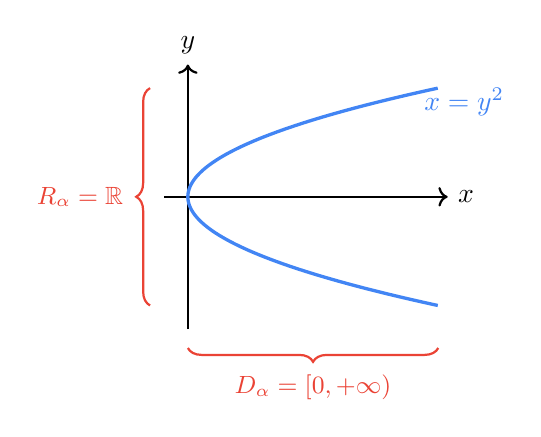
\begin{tikzpicture}[scale=0.6]
  \draw[->, thick] (-0.5,0) -- (5.5,0) node[right] {$x$};
  \draw[->, thick] (0,-2.8) -- (0,2.8) node[above] {$y$};
  \draw[setA, very thick, domain=-2.3:2.3, samples=100] plot ({(\x)^2}, \x);
  \node[setA, right] at (4.8, 2) {$x = y^2$};
  % Braces for D and R
  \draw[thick, setB, decorate, decoration={brace, amplitude=5pt, mirror}]
    (0,-3.2) -- (5.3,-3.2) node[midway, below=6pt, setB] {\small $D_\alpha = [0,+\infty)$};
  \draw[thick, setB, decorate, decoration={brace, amplitude=5pt}]
    (-0.8,-2.3) -- (-0.8,2.3) node[midway, left=6pt, setB] {\small $R_\alpha = \R$};
\end{tikzpicture}
\end{center}

%────────────────────────────────────────
\subsection*{(d)\; $\alpha = \{(x,y) \in \R^2 \mid x^2 + y^2 \le 16\}$}

This is a closed disk of radius~4 centred at the origin.
For any $x$ with $|x| \le 4$, there exists $y$ satisfying $x^2 + y^2 \le 16$, and vice versa.

\begin{answerbox}
$D_\alpha = [-4,\, 4], \qquad R_\alpha = [-4,\, 4].$
\end{answerbox}

\begin{center}
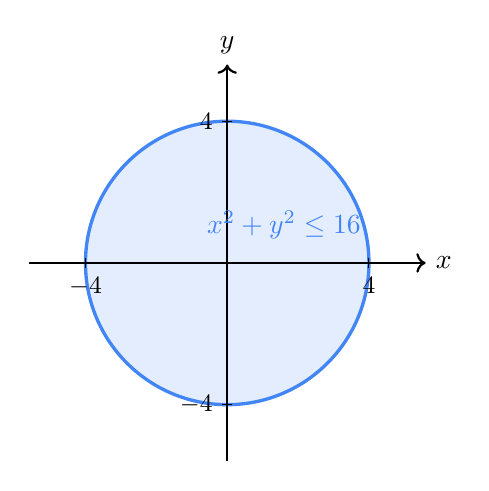
\begin{tikzpicture}[scale=0.6]
  \fill[setA!15] (0,0) circle (3);
  \draw[setA, very thick] (0,0) circle (3);
  \draw[->, thick] (-4.2,0) -- (4.2,0) node[right] {$x$};
  \draw[->, thick] (0,-4.2) -- (0,4.2) node[above] {$y$};
  \foreach \v/\lab in {-3/{-4}, 3/4} {
    \draw (\v, 0.1) -- (\v, -0.1) node[below]{\small $\lab$};
    \draw (0.1, \v) -- (-0.1, \v) node[left]{\small $\lab$};
  }
  \node[setA] at (1.2, 0.8) {$x^2+y^2 \le 16$};
\end{tikzpicture}
\end{center}

%────────────────────────────────────────
\subsection*{(e)\; $\alpha = \{(x,y) \in \N^2 \mid x \mid y\}$}

Here $x \mid y$ means ``$x$ divides $y$.''
Every $x \in \N$ divides some $y$ (e.g.\ $y = x$), so $D_\alpha = \N$.
Every $y \in \N$ is divided by some $x$ (e.g.\ $x = 1$), so $R_\alpha = \N$.

\begin{answerbox}
$D_\alpha = \N, \quad R_\alpha = \N.$
\end{answerbox}

%────────────────────────────────────────
\subsection*{(f)\; $\alpha = \{(x,y) \in \N^2 \mid y \mid x\}$}

This is the inverse of part~(e).  By the same reasoning:

\begin{answerbox}
$D_\alpha = \N, \quad R_\alpha = \N.$
\end{answerbox}

%────────────────────────────────────────
\subsection*{(g)\; $\alpha = \{(x,y) \in \R^2 \mid x + y \le 0\}$}

This is the half-plane below and including the line $y = -x$.
For any $x \in \R$, choose $y = -x - 1$; then $x + y = -1 \le 0$.
For any $y \in \R$, choose $x = -y - 1$.

\begin{answerbox}
$D_\alpha = \R, \quad R_\alpha = \R.$
\end{answerbox}

\begin{center}
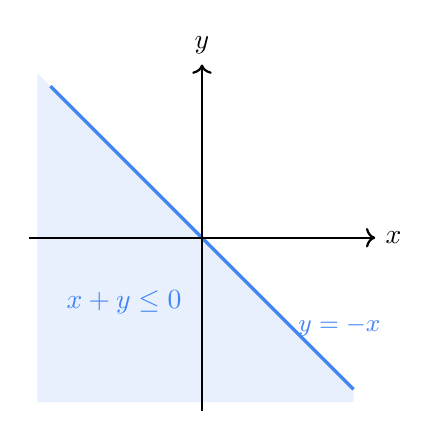
\begin{tikzpicture}[scale=0.55]
  % Shaded half-plane
  \fill[setA!12] (-3.5,3.5) -- (3.5,-3.5) -- (3.5,-3.8) -- (-3.8,-3.8) -- (-3.8,3.8) -- (-3.5,3.5);
  % Boundary line
  \draw[setA, very thick] (-3.5,3.5) -- (3.5,-3.5);
  % Axes
  \draw[->, thick] (-4,0) -- (4,0) node[right] {$x$};
  \draw[->, thick] (0,-4) -- (0,4) node[above] {$y$};
  \node[setA] at (-1.8, -1.5) {$x+y \le 0$};
  \node[setA, above right] at (2, -2.5) {\small $y=-x$};
\end{tikzpicture}
\end{center}

%────────────────────────────────────────
\subsection*{(h)\; $\alpha = \{(x,y) \in \R^2 \mid 2x \ge 3y\}$}

Equivalently $y \le \tfrac{2}{3}\,x$.
For any $x$, choose $y = 0$ (when $x \ge 0$) or any sufficiently small $y$.
For any $y$, choose $x = \tfrac{3}{2}y$.

\begin{answerbox}
$D_\alpha = \R, \quad R_\alpha = \R.$
\end{answerbox}

% ══════════════════════════════════════════════════════════════════
\newpage
\section{Problem 2.1 --- Graph and Matrix of Relations}
% ══════════════════════════════════════════════════════════════════

\begin{theorybox}[Graphs and Matrices of Relations]
Let $\alpha$ be a relation on a finite set $A = \{a_1,\dots,a_n\}$.
\begin{itemize}[nosep]
  \item \textbf{Graph:} Each element of $A$ is a vertex.  For a symmetric relation, if $(a_i, a_j) \in \alpha$ with $i \ne j$, draw an \emph{undirected} edge between $a_i$ and $a_j$.
  \item \textbf{Matrix:} The $n \times n$ matrix $M$ with $M_{ij} = 1$ if $(a_i, a_j) \in \alpha$, and $M_{ij} = 0$ otherwise.  For a symmetric relation $M = M^T$.
\end{itemize}
\end{theorybox}

\begin{problembox}
Construct the graph and matrix for the following relations on $A = \{a, b, c, d, e\}$.
\end{problembox}

% TikZ style for undirected graph nodes
\tikzset{
  gnode/.style={circle, draw, thick, minimum size=8mm, inner sep=0pt, font=\small},
}

%────────────────────────────────────────
\subsection*{(a)\; $\alpha = \{(a,b),(b,a),(b,c),(c,b),(c,a),(a,c),(d,e),(e,d)\}$}

Since every pair appears with its reverse, the relation is symmetric. Undirected edges:
\[
  \boxed{a\text{--}b,\quad b\text{--}c,\quad a\text{--}c,\quad d\text{--}e.}
\]

\begin{center}
\begin{minipage}{0.45\textwidth}\centering
\begin{tikzpicture}
  % Pentagon layout
  \node[gnode] (a) at (90:1.8)  {$a$};
  \node[gnode] (b) at (18:1.8)  {$b$};
  \node[gnode] (c) at (306:1.8) {$c$};
  \node[gnode] (d) at (234:1.8) {$d$};
  \node[gnode] (e) at (162:1.8) {$e$};

  \draw[thick, setA] (a) -- (b);
  \draw[thick, setA] (b) -- (c);
  \draw[thick, setA] (a) -- (c);
  \draw[thick, setA] (d) -- (e);
\end{tikzpicture}
\end{minipage}%
\begin{minipage}{0.5\textwidth}\centering
\textbf{Color-coded matrix} (symmetry visible):\\[4pt]
{\small Diagonal = \colorbox{diagGray}{gray},\;
mirrored 1's = \colorbox{mirrorBlue}{blue} / \colorbox{mirrorRose}{rose}.}\\[4pt]
\renewcommand{\arraystretch}{1.15}
$M_\alpha = \left(\;\begin{tabular}{c|ccccc}
  & $a$ & $b$ & $c$ & $d$ & $e$ \\\hline
$a$ & \cellcolor{diagGray}0 & \cellcolor{mirrorBlue}1 & \cellcolor{mirrorRose}1 & 0 & 0 \\
$b$ & \cellcolor{mirrorBlue}1 & \cellcolor{diagGray}0 & \cellcolor{mirrorBlue}1 & 0 & 0 \\
$c$ & \cellcolor{mirrorRose}1 & \cellcolor{mirrorBlue}1 & \cellcolor{diagGray}0 & 0 & 0 \\
$d$ & 0 & 0 & 0 & \cellcolor{diagGray}0 & \cellcolor{mirrorRose}1 \\
$e$ & 0 & 0 & 0 & \cellcolor{mirrorRose}1 & \cellcolor{diagGray}0
\end{tabular}\;\right)$
\end{minipage}
\end{center}

The matrix is symmetric ($M = M^T$): every shaded 1 above the diagonal has a matching shaded 1 below it.
Two connected components: the triangle $\{a,b,c\}$ and the edge $\{d,e\}$.

\textbf{Construction order.}\; For a finite relation on $A$: (1) list the ordered pairs, (2) fill the matrix row by row from the pairs, (3) read the directed graph off the matrix.

%────────────────────────────────────────
\subsection*{(b)\; $\alpha = \{(a,b),(b,a),(b,c),(c,b),(c,d),(d,c),(c,a),(a,c)\}$}

Undirected edges:
\[
  \boxed{a\text{--}b,\quad b\text{--}c,\quad c\text{--}d,\quad a\text{--}c.}
\]

\begin{center}
\begin{minipage}{0.45\textwidth}\centering
\begin{tikzpicture}
  \node[gnode] (a) at (90:1.8)  {$a$};
  \node[gnode] (b) at (18:1.8)  {$b$};
  \node[gnode] (c) at (306:1.8) {$c$};
  \node[gnode] (d) at (234:1.8) {$d$};
  \node[gnode] (e) at (162:1.8) {$e$};

  \draw[thick, setA] (a) -- (b);
  \draw[thick, setA] (b) -- (c);
  \draw[thick, setA] (a) -- (c);
  \draw[thick, setA] (c) -- (d);
\end{tikzpicture}
\end{minipage}%
\begin{minipage}{0.5\textwidth}\centering
\renewcommand{\arraystretch}{1.15}
$M_\alpha = \left(\;\begin{tabular}{c|ccccc}
  & $a$ & $b$ & $c$ & $d$ & $e$ \\\hline
$a$ & \cellcolor{diagGray}0 & \cellcolor{mirrorBlue}1 & \cellcolor{mirrorRose}1 & 0 & 0 \\
$b$ & \cellcolor{mirrorBlue}1 & \cellcolor{diagGray}0 & \cellcolor{mirrorBlue}1 & 0 & 0 \\
$c$ & \cellcolor{mirrorRose}1 & \cellcolor{mirrorBlue}1 & \cellcolor{diagGray}0 & \cellcolor{mirrorRose}1 & 0 \\
$d$ & 0 & 0 & \cellcolor{mirrorRose}1 & \cellcolor{diagGray}0 & 0 \\
$e$ & 0 & 0 & 0 & 0 & \cellcolor{diagGray}0
\end{tabular}\;\right)$
\end{minipage}
\end{center}

Triangle $\{a,b,c\}$ with $d$ attached to~$c$; vertex~$e$ is isolated.

%────────────────────────────────────────
\subsection*{(c)}

Part~(c) is identical to part~(b) in the original problem sheet.  The graph and matrix are the same as above.

% ══════════════════════════════════════════════════════════════════
\newpage
\section{Problem 2.2 --- Digraph and Matrix of Relations}
% ══════════════════════════════════════════════════════════════════

\begin{theorybox}[Directed Graphs (Digraphs)]
For a (not necessarily symmetric) relation $\alpha$ on $A$:
\begin{itemize}[nosep]
  \item \textbf{Digraph:} Vertices are elements of $A$.  For each $(a_i,a_j) \in \alpha$, draw an arrow $a_i \to a_j$.  A pair $(a_i,a_i)$ is a \emph{loop}.
  \item \textbf{Matrix:} Same construction; the matrix need not be symmetric.
\end{itemize}
\end{theorybox}

\begin{problembox}
Construct the digraph and matrix for the following relations on $A = \{a, b, c, d, e, f\}$.
\end{problembox}

% TikZ style for digraph
\tikzset{
  dnode/.style={circle, draw, thick, minimum size=8mm, inner sep=0pt, font=\small},
  darr/.style={-{Stealth[length=5pt]}, thick, setA},
}

%────────────────────────────────────────
\subsection*{(a)\; $\alpha = \{(a,b),(b,c),(a,c),(b,e),(c,f),(c,d),(d,f),(f,e)\}$}

\begin{center}
\begin{tikzpicture}
  % Layout: top-flow for a→b→c, bottom for e,f,d
  \node[dnode] (a) at (0,2.5)   {$a$};
  \node[dnode] (b) at (2.5,2.5) {$b$};
  \node[dnode] (c) at (5,2.5)   {$c$};
  \node[dnode] (f) at (2.5,0)   {$f$};
  \node[dnode] (e) at (0,0)     {$e$};
  \node[dnode] (d) at (5,0)     {$d$};

  \draw[darr] (a) -- (b);
  \draw[darr] (b) -- (c);
  \draw[darr] (a) edge[bend right=15] (c);
  \draw[darr] (b) edge[bend left=8] (e);
  \draw[darr] (c) -- (f);
  \draw[darr] (c) -- (d);
  \draw[darr] (d) -- (f);
  \draw[darr] (f) -- (e);
\end{tikzpicture}
\end{center}

\[
M_\alpha = \bordermatrix{
  & a & b & c & d & e & f \cr
a & 0 & 1 & 1 & 0 & 0 & 0 \cr
b & 0 & 0 & 1 & 0 & 1 & 0 \cr
c & 0 & 0 & 0 & 1 & 0 & 1 \cr
d & 0 & 0 & 0 & 0 & 0 & 1 \cr
e & 0 & 0 & 0 & 0 & 0 & 0 \cr
f & 0 & 0 & 0 & 0 & 1 & 0 \cr
}
\]

%────────────────────────────────────────
\subsection*{(b)\; $\alpha = \{(a,b),(b,c),(d,c),(d,e),(f,e),(f,a),(b,e)\}$}

\begin{center}
\begin{tikzpicture}
  \node[dnode] (a) at (0,2.5)   {$a$};
  \node[dnode] (b) at (2.5,2.5) {$b$};
  \node[dnode] (c) at (5,2.5)   {$c$};
  \node[dnode] (d) at (5,0)     {$d$};
  \node[dnode] (e) at (2.5,0)   {$e$};
  \node[dnode] (f) at (0,0)     {$f$};

  \draw[darr] (a) -- (b);
  \draw[darr] (b) -- (c);
  \draw[darr] (b) -- (e);
  \draw[darr] (d) -- (c);
  \draw[darr] (d) -- (e);
  \draw[darr] (f) -- (e);
  \draw[darr] (f) -- (a);
\end{tikzpicture}
\end{center}

\[
M_\alpha = \bordermatrix{
  & a & b & c & d & e & f \cr
a & 0 & 1 & 0 & 0 & 0 & 0 \cr
b & 0 & 0 & 1 & 0 & 1 & 0 \cr
c & 0 & 0 & 0 & 0 & 0 & 0 \cr
d & 0 & 0 & 1 & 0 & 1 & 0 \cr
e & 0 & 0 & 0 & 0 & 0 & 0 \cr
f & 1 & 0 & 0 & 0 & 1 & 0 \cr
}
\]

%────────────────────────────────────────
\subsection*{(c)\; $\alpha = \{(a,c),(c,c),(c,d),(c,e),(e,c),(e,e),(e,f),(a,e)\}$}

\begin{center}
\begin{tikzpicture}
  % Reposition: b is isolated, push it aside; cluster active vertices
  \node[dnode] (a) at (0,2)     {$a$};
  \node[dnode] (c) at (3,2)     {$c$};
  \node[dnode] (d) at (5.5,2)   {$d$};
  \node[dnode] (e) at (3,0)     {$e$};
  \node[dnode] (f) at (5.5,0)   {$f$};
  \node[dnode, dashed, gray] (b) at (0,0) {$b$};

  \draw[darr] (a) -- (c);
  \draw[darr] (a) -- (e);
  \draw[darr] (c) edge[loop above, looseness=8, min distance=10mm] (c);
  \draw[darr] (c) -- (d);
  \draw[darr] (c) edge[bend left=12] (e);
  \draw[darr] (e) edge[bend left=12] (c);
  \draw[darr] (e) edge[loop below, looseness=8, min distance=10mm] (e);
  \draw[darr] (e) -- (f);
\end{tikzpicture}
\end{center}

Note: vertex~$b$ (dashed) is completely isolated --- no edges touch it.

\[
M_\alpha = \bordermatrix{
  & a & b & c & d & e & f \cr
a & 0 & 0 & 1 & 0 & 1 & 0 \cr
b & 0 & 0 & 0 & 0 & 0 & 0 \cr
c & 0 & 0 & 1 & 1 & 1 & 0 \cr
d & 0 & 0 & 0 & 0 & 0 & 0 \cr
e & 0 & 0 & 1 & 0 & 1 & 1 \cr
f & 0 & 0 & 0 & 0 & 0 & 0 \cr
}
\]

The loops at $c$ and $e$ appear as 1's on the main diagonal.  The $b$-row and $b$-column are all zeros.

A zero row in the matrix means ``no outgoing edges'' from that element. A zero column means ``no incoming edges'' to that element.

%────────────────────────────────────────
\subsection*{Contrast: Symmetric (2.1) vs.\ Non-symmetric (2.2) Matrices}

The matrices from Problems~2.1 and 2.2 illustrate the structural difference between symmetric (undirected) and general (directed) relations.  Below we place the matrix from~2.1\,(a) next to the matrix from~2.2\,(a):

\begin{center}
\begin{minipage}{0.45\textwidth}\centering
\textbf{Problem 2.1\,(a) --- Symmetric}\\[4pt]
\renewcommand{\arraystretch}{1.15}
$\left(\;\begin{tabular}{ccccc}
0 & 1 & 1 & 0 & 0 \\
1 & 0 & 1 & 0 & 0 \\
1 & 1 & 0 & 0 & 0 \\
0 & 0 & 0 & 0 & 1 \\
0 & 0 & 0 & 1 & 0
\end{tabular}\;\right)$\\[4pt]
{\small $M = M^T$: entry $(i,j)$ always equals entry $(j,i)$.\\
Undirected edges; no arrows needed.}
\end{minipage}%
\hfill
\begin{minipage}{0.45\textwidth}\centering
\textbf{Problem 2.2\,(a) --- Non-symmetric}\\[4pt]
\renewcommand{\arraystretch}{1.15}
$\left(\;\begin{tabular}{cccccc}
0 & 1 & 1 & 0 & 0 & 0 \\
0 & 0 & 1 & 0 & 1 & 0 \\
0 & 0 & 0 & 1 & 0 & 1 \\
0 & 0 & 0 & 0 & 0 & 1 \\
0 & 0 & 0 & 0 & 0 & 0 \\
0 & 0 & 0 & 0 & 1 & 0
\end{tabular}\;\right)$\\[4pt]
{\small $M \ne M^T$: e.g.\ $M_{12}=1$ but $M_{21}=0$.\\
Directed edges (arrows) required.}
\end{minipage}
\end{center}

%────────────────────────────────────────
\subsection*{Degree Tracking --- Problem 2.2\,(a)}

For a directed relation, each vertex has an \textbf{in-degree} (number of incoming edges) and an \textbf{out-degree} (number of outgoing edges).  These are read directly from the matrix: the out-degree of vertex~$v$ is the row sum, and the in-degree is the column sum.

\begin{center}
\renewcommand{\arraystretch}{1.2}
\begin{tabular}{c|c|c}
  \toprule
  \textbf{Vertex} & \textbf{In-degree} & \textbf{Out-degree} \\
  \midrule
  $a$ & 0 & 2 \\
  $b$ & 1 & 2 \\
  $c$ & 2 & 2 \\
  $d$ & 1 & 1 \\
  $e$ & 2 & 0 \\
  $f$ & 2 & 1 \\
  \bottomrule
\end{tabular}
\end{center}

Observe that $\sum \text{in-degrees} = \sum \text{out-degrees} = |\alpha| = 8$ (every edge contributes~1 to each total).

Vertex~$e$ has out-degree~0, making it a \emph{sink} (no outgoing arrows).
Vertex~$a$ has in-degree~0, making it a \emph{source} (no incoming arrows).

% ══════════════════════════════════════════════════════════════════
\newpage
\section{Problem 3.3 --- Composition of Relations}
% ══════════════════════════════════════════════════════════════════

\begin{theorybox}[Composition of Relations]
Let $\alpha \subseteq A \times B$ and $\beta \subseteq B \times C$.  The \textbf{composition} $\alpha \circ \beta$ (also written $\alpha \cdot \beta$) is the relation on $A \times C$ defined by:
\[
  (x, z) \in \alpha \circ \beta
  \;\;\Longleftrightarrow\;\;
  \exists\, y \in B:\;
  (x, y) \in \alpha \;\land\; (y, z) \in \beta.
\]
Read left-to-right: first go through $\alpha$ (from $x$ to some $y$), then through $\beta$ (from $y$ to $z$).
\end{theorybox}

\begin{problembox}
Let $\alpha$ and $\beta$ be relations on $\Z$:
\[
  \alpha = \{(x,\, x+2) \mid x \in \Z\}, \qquad
  \beta  = \{(x,\, x^2) \mid x \in \Z\}.
\]
Find $\alpha \circ \beta$ and $\beta \circ \alpha$.
\end{problembox}

\textbf{Convention.}\; Relation composition is read \textbf{left-to-right} here: in $\alpha \circ \beta$, apply $\alpha$ first, then $\beta$. This is the most common source of errors.

\medskip

\subsection*{Finding $\alpha \circ \beta$}

We apply $\alpha$ first, then $\beta$:
\begin{itemize}[nosep]
  \item $(x, y) \in \alpha \;\Longrightarrow\; y = x + 2$.
  \item $(y, z) \in \beta  \;\Longrightarrow\; z = y^2 = (x+2)^2$.
\end{itemize}

\begin{answerbox}
$\alpha \circ \beta = \{\,(x,\; (x+2)^2) \mid x \in \Z\,\}
                    = \{\,(x,\; x^2 + 4x + 4) \mid x \in \Z\,\}.$
\end{answerbox}

\subsection*{Finding $\beta \circ \alpha$}

We apply $\beta$ first, then $\alpha$:
\begin{itemize}[nosep]
  \item $(x, y) \in \beta  \;\Longrightarrow\; y = x^2$.
  \item $(y, z) \in \alpha \;\Longrightarrow\; z = y + 2 = x^2 + 2$.
\end{itemize}

\begin{answerbox}
$\beta \circ \alpha = \{\,(x,\; x^2 + 2) \mid x \in \Z\,\}.$
\end{answerbox}

\subsection*{Verification and comparison}

\begin{center}
\renewcommand{\arraystretch}{1.1}
\begin{tabular}{r c c}
  \toprule
  $x$ & $\alpha \circ \beta$: $(x+2)^2$ & $\beta \circ \alpha$: $x^2+2$ \\
  \midrule
  $-2$ & $0$ & $6$ \\
  $0$  & $4$ & $2$ \\
  $1$  & $9$ & $3$ \\
  $3$  & $25$ & $11$ \\
  \bottomrule
\end{tabular}
\end{center}

\textbf{Key observation:} $\boxed{\alpha \circ \beta \ne \beta \circ \alpha}$\,--- composition of relations is \emph{not commutative} in general.

\begin{center}
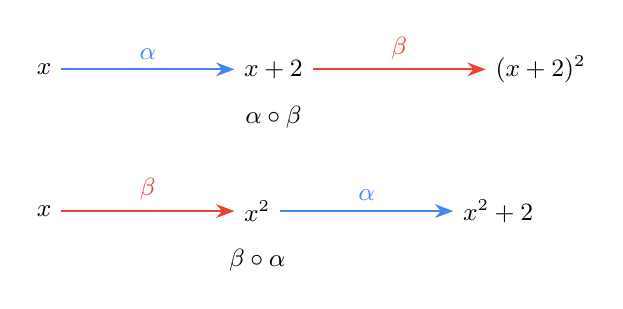
\begin{tikzpicture}[>=Stealth, font=\small, node distance=2.2cm]
  % alpha then beta
  \node (x1) {$x$};
  \node[right=of x1] (y1) {$x+2$};
  \node[right=of y1] (z1) {$(x+2)^2$};
  \draw[->, thick, setA] (x1) -- node[above]{$\alpha$} (y1);
  \draw[->, thick, setB] (y1) -- node[above]{$\beta$} (z1);
  \node[below=3pt of y1] {\small $\alpha \circ \beta$};

  % beta then alpha
  \begin{scope}[yshift=-1.8cm]
  \node (x2) {$x$};
  \node[right=of x2] (y2) {$x^2$};
  \node[right=of y2] (z2) {$x^2+2$};
  \draw[->, thick, setB] (x2) -- node[above]{$\beta$} (y2);
  \draw[->, thick, setA] (y2) -- node[above]{$\alpha$} (z2);
  \node[below=3pt of y2] {\small $\beta \circ \alpha$};
  \end{scope}
\end{tikzpicture}
\end{center}

\subsection*{Mapping Diagram for a Finite Example}

To build further intuition, consider a concrete finite example.
Let $X = \{1,2,3\}$, $Y = \{a,b\}$, $Z = \{p,q\}$, with
\[
  R = \{(1,a),\;(2,b),\;(3,a)\} \subseteq X \times Y,
  \qquad
  S = \{(a,p),\;(b,q)\} \subseteq Y \times Z.
\]
Then $S \circ R$ connects each $x \in X$ to every $z \in Z$ reachable via some intermediate $y$:
\[
  \boxed{S \circ R = \{(1,p),\;(2,q),\;(3,p)\}.}
\]

\begin{center}
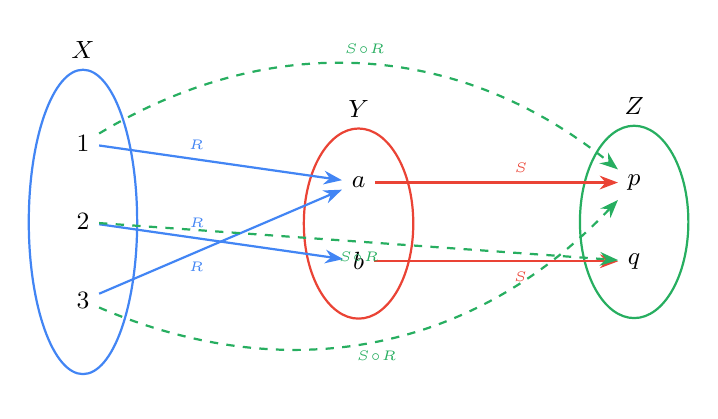
\begin{tikzpicture}[>=Stealth, node distance=0.8cm, font=\small]
  % Set X
  \node (x1) at (0, 2)   {$1$};
  \node (x2) at (0, 1)   {$2$};
  \node (x3) at (0, 0)   {$3$};
  \node[draw=setA, ellipse, thick, fit=(x1)(x2)(x3),
        inner xsep=8pt, inner ysep=4pt, label={above:$X$}] {};

  % Set Y
  \node (ya) at (3.5, 1.5) {$a$};
  \node (yb) at (3.5, 0.5) {$b$};
  \node[draw=setB, ellipse, thick, fit=(ya)(yb),
        inner xsep=8pt, inner ysep=4pt, label={above:$Y$}] {};

  % Set Z
  \node (zp) at (7, 1.5) {$p$};
  \node (zq) at (7, 0.5) {$q$};
  \node[draw=newEdge, ellipse, thick, fit=(zp)(zq),
        inner xsep=8pt, inner ysep=4pt, label={above:$Z$}] {};

  % Relation R (X -> Y)
  \draw[->, thick, setA] (x1) -- node[above, pos=0.4]{\tiny $R$} (ya);
  \draw[->, thick, setA] (x2) -- node[above, pos=0.4]{\tiny $R$} (yb);
  \draw[->, thick, setA] (x3) -- node[below, pos=0.4]{\tiny $R$} (ya);

  % Relation S (Y -> Z)
  \draw[->, thick, setB] (ya) -- node[above, pos=0.6]{\tiny $S$} (zp);
  \draw[->, thick, setB] (yb) -- node[below, pos=0.6]{\tiny $S$} (zq);

  % Composition paths (dashed, green)
  \draw[->, thick, newEdge, dashed, bend left=35]
    (x1) to node[above, pos=0.5]{\tiny $S\!\circ\!R$} (zp);
  \draw[->, thick, newEdge, dashed, bend right=0]
    (x2) to node[below, pos=0.5]{\tiny $S\!\circ\!R$} (zq);
  \draw[->, thick, newEdge, dashed, bend right=35]
    (x3) to node[below, pos=0.5]{\tiny $S\!\circ\!R$} (zp);
\end{tikzpicture}
\end{center}

{\small\textbf{Reading the diagram:} Solid blue arrows are~$R$, solid red arrows are~$S$, and dashed green arrows are the composed pairs in $S \circ R$.  Each dashed arrow represents a connected path through some intermediate vertex in~$Y$.}

% ══════════════════════════════════════════════════════════════════
\newpage
\section{Problem 4.1 --- Properties of Relations}
% ══════════════════════════════════════════════════════════════════

\begin{theorybox}[Properties of Relations]
A relation $\alpha$ on a set $A$ may satisfy:
\begin{itemize}[nosep]
  \item \textbf{Reflexive:} $\forall x \in A:\; (x,x) \in \alpha$.
  \item \textbf{Symmetric:} $(x,y) \in \alpha \;\Rightarrow\; (y,x) \in \alpha$.
  \item \textbf{Antisymmetric:} $(x,y) \in \alpha \;\land\; (y,x) \in \alpha \;\Rightarrow\; x = y$.
  \item \textbf{Transitive:} $(x,y) \in \alpha \;\land\; (y,z) \in \alpha \;\Rightarrow\; (x,z) \in \alpha$.
\end{itemize}
Note that symmetric and antisymmetric are \emph{not} negations of each other --- a relation can be both (e.g.\ $\Delta_A$) or neither.
\end{theorybox}

\begin{problembox}
Determine which properties each of the following relations possesses.
\end{problembox}

%────────────────────────────────────────
\subsection*{(a)\; $\alpha = \{(x,y) \in \R^2 \mid x^2 + y^2 = 1\}$}

Geometrically, $(x,y) \in \alpha$ iff the point $(x,y)$ lies on the unit circle.

\begin{center}
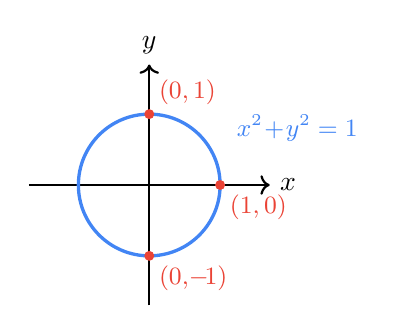
\begin{tikzpicture}[scale=0.9]
  \draw[->, thick] (-1.7,0) -- (1.7,0) node[right] {$x$};
  \draw[->, thick] (0,-1.7) -- (0,1.7) node[above] {$y$};
  \draw[setA, very thick] (0,0) circle (1);
  \fill[setB] (1,0) circle (2pt) node[below right]{\small $(1,0)$};
  \fill[setB] (0,1) circle (2pt) node[above right]{\small $(0,1)$};
  \fill[setB] (0,-1) circle (2pt) node[below right]{\small $(0,\!-\!1)$};
  \node[setA, right] at (1.1, 0.8) {\small $x^2\!+\!y^2=1$};
\end{tikzpicture}
\end{center}

\textbf{Reflexive?} No.  We'd need $2x^2 = 1$ for \emph{all} $x$, which fails for $x = 0$.

\textbf{Symmetric?} Yes.  $x^2 + y^2 = y^2 + x^2$. \checkmark

\textbf{Antisymmetric?} No.  $(0, 1) \in \alpha$ and $(1, 0) \in \alpha$, but $0 \ne 1$.

\textbf{Transitive?} No.  $(1, 0)$ and $(0, 1) \in \alpha$, but $(1, 1) \notin \alpha$ since $1 + 1 = 2 \ne 1$.

\begin{answerbox}
Symmetric only.
\end{answerbox}

\begin{center}
\renewcommand{\arraystretch}{1.15}
\begin{tabular}{l|c|l}
  \toprule
  \textbf{Property} & \textbf{Holds?} & \textbf{Justification} \\
  \midrule
  Reflexive      & No  & $(0,0)$: $0^2+0^2=0\ne1$ \\
  Symmetric      & Yes & $x^2+y^2 = y^2+x^2$ \\
  Antisymmetric  & No  & $(0,1)$ and $(1,0)$ both $\in\alpha$, but $0\ne1$ \\
  Transitive     & No  & $(1,0),(0,1)\in\alpha$ but $(1,1)\notin\alpha$ \\
  \midrule
  \textbf{Classification} & \multicolumn{2}{l}{Neither equivalence relation nor partial order} \\
  \bottomrule
\end{tabular}
\end{center}

%────────────────────────────────────────
\subsection*{(b)\; $\alpha = \{(x,y) \in \R^2 \mid x^2 = y^2\}$}

Equivalently $|x| = |y|$, so $y = \pm x$.

\textbf{Reflexive?} Yes.  $x^2 = x^2$ always holds. \checkmark

\textbf{Symmetric?} Yes.  $x^2 = y^2 \Rightarrow y^2 = x^2$. \checkmark

\textbf{Antisymmetric?} No.  $1^2 = (-1)^2$ and $(-1)^2 = 1^2$, but $1 \ne -1$.

\textbf{Transitive?} Yes.  $x^2 = y^2$ and $y^2 = z^2$ imply $x^2 = z^2$. \checkmark

\begin{answerbox}
Reflexive, symmetric, transitive --- this is an \textbf{equivalence relation}.

Equivalence classes: $[x] = \{x, -x\}$ for each $x \in \R$.
\end{answerbox}

\begin{center}
\renewcommand{\arraystretch}{1.15}
\begin{tabular}{l|c|l}
  \toprule
  \textbf{Property} & \textbf{Holds?} & \textbf{Justification} \\
  \midrule
  Reflexive      & Yes & $x^2 = x^2$ always \\
  Symmetric      & Yes & $x^2=y^2 \Rightarrow y^2=x^2$ \\
  Antisymmetric  & No  & $1^2=(-1)^2$ and $(-1)^2=1^2$, but $1\ne -1$ \\
  Transitive     & Yes & $x^2=y^2, y^2=z^2 \Rightarrow x^2=z^2$ \\
  \midrule
  \textbf{Classification} & \multicolumn{2}{l}{\textbf{Equivalence relation}} \\
  \bottomrule
\end{tabular}
\end{center}

\smallskip
\textbf{Induced partition:}\; $\R$ is partitioned into blocks $\{x,-x\}$.  For $x=0$ the block is $\{0\}$; for $x\ne 0$ each block has exactly two elements.

%────────────────────────────────────────
\subsection*{(c)\; $\alpha = \{(x,y) \in \Z^2 \mid x \mid y\}$}

Here $x \mid y$ means ``$x$ divides $y$,'' i.e.\ $\exists\, k \in \Z:\; y = kx$.

\textbf{Reflexive?} Yes.  $x = 1 \cdot x$, so $x \mid x$ for all $x \in \Z$. \checkmark

\textbf{Symmetric?} No.  $1 \mid 2$ but $2 \nmid 1$.

\textbf{Antisymmetric?} No (on $\Z$!).  We have $2 \mid (-2)$ and $(-2) \mid 2$, but $2 \ne -2$.

\textbf{Transitive?} Yes.  If $y = kx$ and $z = \ell y$, then $z = \ell k x$, so $x \mid z$. \checkmark

\begin{answerbox}
Reflexive and transitive, but \emph{not} antisymmetric on $\Z$ (due to sign).
\end{answerbox}

\begin{center}
\renewcommand{\arraystretch}{1.15}
\begin{tabular}{l|c|l}
  \toprule
  \textbf{Property} & \textbf{Holds?} & \textbf{Justification} \\
  \midrule
  Reflexive      & Yes & $x = 1\cdot x$ \\
  Symmetric      & No  & $1\mid 2$ but $2\nmid 1$ \\
  Antisymmetric  & No  & $2\mid(-2)$ and $(-2)\mid 2$, but $2\ne -2$ \\
  Transitive     & Yes & $y=kx,\; z=\ell y \Rightarrow z=\ell k x$ \\
  \midrule
  \textbf{Classification} & \multicolumn{2}{l}{Preorder (reflexive + transitive), not a partial order} \\
  \bottomrule
\end{tabular}
\end{center}

%────────────────────────────────────────
\subsection*{(d)\; $\alpha = \{(x,y) \in \N^2 \mid x \mid y\}$}

Same as (c) but restricted to $\N = \{1, 2, 3, \dots\}$ (positive integers).

\textbf{Reflexive?} Yes.  $x = 1 \cdot x$. \checkmark

\textbf{Symmetric?} No.  $1 \mid 2$ but $2 \nmid 1$.

\textbf{Antisymmetric?} Yes.  If $x \mid y$ and $y \mid x$ with $x, y > 0$: then $y = kx$ and $x = \ell y$ with $k, \ell \ge 1$, so $x = k\ell\, x$ giving $k\ell = 1$, hence $k = \ell = 1$ and $x = y$. \checkmark

\textbf{Transitive?} Yes (same argument as~(c)). \checkmark

\begin{answerbox}
Reflexive, antisymmetric, transitive --- this is a \textbf{partial order}.

Compare with (c): restricting from $\Z$ to $\N$ restores antisymmetry.
\end{answerbox}

\begin{center}
\renewcommand{\arraystretch}{1.15}
\begin{tabular}{l|c|l}
  \toprule
  \textbf{Property} & \textbf{Holds?} & \textbf{Justification} \\
  \midrule
  Reflexive      & Yes & $x = 1\cdot x$ \\
  Symmetric      & No  & $1\mid 2$ but $2\nmid 1$ \\
  Antisymmetric  & Yes & $x\mid y,\; y\mid x$ with $x,y>0 \Rightarrow x=y$ \\
  Transitive     & Yes & $y=kx,\; z=\ell y \Rightarrow z=\ell k x$ \\
  \midrule
  \textbf{Classification} & \multicolumn{2}{l}{\textbf{Partial order} $(\N, \mid)$} \\
  \bottomrule
\end{tabular}
\end{center}

%────────────────────────────────────────
\subsection*{(e)\; $\alpha = \{(x,y) \in \N^2 \mid \gcd(x,y) = 1\}$}

$(x,y) \in \alpha$ iff $x$ and $y$ are coprime.

\textbf{Reflexive?} No.  $\gcd(2,2) = 2 \ne 1$.

\textbf{Symmetric?} Yes.  $\gcd(x,y) = \gcd(y,x)$. \checkmark

\textbf{Antisymmetric?} No.  $\gcd(2,3) = 1$ and $\gcd(3,2) = 1$, but $2 \ne 3$.

\textbf{Transitive?} No.  $\gcd(2,3) = 1$ and $\gcd(3,4) = 1$, but $\gcd(2,4) = 2 \ne 1$.

\begin{answerbox}
Symmetric only.
\end{answerbox}

\begin{center}
\renewcommand{\arraystretch}{1.15}
\begin{tabular}{l|c|l}
  \toprule
  \textbf{Property} & \textbf{Holds?} & \textbf{Justification} \\
  \midrule
  Reflexive      & No  & $\gcd(2,2)=2\ne 1$ \\
  Symmetric      & Yes & $\gcd(x,y)=\gcd(y,x)$ \\
  Antisymmetric  & No  & $\gcd(2,3)=1$ and $\gcd(3,2)=1$, but $2\ne 3$ \\
  Transitive     & No  & $\gcd(2,3)=1,\;\gcd(3,4)=1$, but $\gcd(2,4)=2$ \\
  \midrule
  \textbf{Classification} & \multicolumn{2}{l}{Neither equivalence relation nor partial order} \\
  \bottomrule
\end{tabular}
\end{center}

%────────────────────────────────────────
\subsection*{(f)\; $\alpha = \{(x,y) \in \Z^2 \mid \gcd(x,y) = 1\}$}

The analysis is identical to part~(e) since $\gcd$ depends only on absolute values.  The same counterexamples apply.

\begin{answerbox}
Symmetric only.
\end{answerbox}

\begin{center}
\renewcommand{\arraystretch}{1.15}
\begin{tabular}{l|c|l}
  \toprule
  \textbf{Property} & \textbf{Holds?} & \textbf{Justification} \\
  \midrule
  Reflexive      & No  & $\gcd(2,2)=2\ne 1$ \\
  Symmetric      & Yes & $\gcd(x,y)=\gcd(y,x)$ \\
  Antisymmetric  & No  & $\gcd(2,3)=1$ and $\gcd(3,2)=1$, but $2\ne 3$ \\
  Transitive     & No  & $\gcd(2,3)=1,\;\gcd(3,4)=1$, but $\gcd(2,4)=2$ \\
  \midrule
  \textbf{Classification} & \multicolumn{2}{l}{Neither equivalence relation nor partial order} \\
  \bottomrule
\end{tabular}
\end{center}

%────────────────────────────────────────
\subsection*{Summary Table}

\begin{center}
\renewcommand{\arraystretch}{1.3}
\begin{tabular}{l c c c c l}
  \toprule
  \textbf{Relation} & \textbf{Refl.} & \textbf{Symm.} & \textbf{Antisymm.} & \textbf{Trans.} & \textbf{Type} \\
  \midrule
  (a)\; $x^2+y^2=1$ on $\R$    & ---  & \checkmark & ---  & --- & --- \\
  (b)\; $x^2=y^2$ on $\R$      & \checkmark & \checkmark & --- & \checkmark & equivalence \\
  (c)\; $x \mid y$ on $\Z$     & \checkmark & --- & --- & \checkmark & preorder \\
  (d)\; $x \mid y$ on $\N$     & \checkmark & --- & \checkmark & \checkmark & partial order \\
  (e)\; $\gcd=1$ on $\N$       & ---  & \checkmark & --- & --- & --- \\
  (f)\; $\gcd=1$ on $\Z$       & ---  & \checkmark & --- & --- & --- \\
  \bottomrule
\end{tabular}
\end{center}

\textbf{How to check (quick tests):}
\begin{itemize}[nosep]
  \item Not reflexive: find one $x$ with $(x,x) \notin R$.
  \item Not symmetric: find $(a,b) \in R$ with $(b,a) \notin R$.
  \item Not antisymmetric: find $a \neq b$ with both $(a,b)$ and $(b,a)$ in $R$.
  \item Not transitive: find $(a,b), (b,c) \in R$ with $(a,c) \notin R$.
\end{itemize}

% ══════════════════════════════════════════════════════════════════
\newpage
\section{Problem 7.2 --- Closures of a Relation}
% ══════════════════════════════════════════════════════════════════

\begin{theorybox}[Closures of a Relation]
Let $\alpha$ be a relation on a finite set $A$.
\begin{itemize}[nosep]
  \item \textbf{Reflexive closure} $r(\alpha) = \alpha \cup \Delta_A$, where $\Delta_A = \{(x,x) \mid x \in A\}$.
  \item \textbf{Symmetric closure} $s(\alpha) = \alpha \cup \alpha^{-1}$, where $\alpha^{-1} = \{(y,x) \mid (x,y) \in \alpha\}$.
  \item \textbf{Transitive closure} $t(\alpha) = \alpha \cup \alpha^2 \cup \alpha^3 \cup \cdots$\; (union of all powers until no new pairs appear).
\end{itemize}
The closure adds the \emph{fewest} pairs needed to acquire the property.
\end{theorybox}

\begin{problembox}
Let $A = \{1, 2, 3, 4\}$ and $\alpha = \{(1,2),\,(3,1),\,(3,2),\,(2,4)\}$.

Find $r(\alpha)$, $s(\alpha)$, and $t(\alpha)$.
\end{problembox}

\subsection*{The original relation}

\begin{center}
\begin{minipage}{0.45\textwidth}\centering
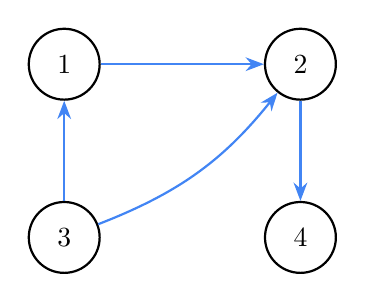
\begin{tikzpicture}[
  every node/.style={circle, draw, thick, minimum size=9mm, inner sep=0pt},
  >=Stealth
]
  \node (1) at (0,2.2)   {$1$};
  \node (2) at (3,2.2)   {$2$};
  \node (3) at (0,0)     {$3$};
  \node (4) at (3,0)     {$4$};

  \draw[->, thick, setA] (1) -- (2);
  \draw[->, thick, setA] (3) -- (1);
  \draw[->, thick, setA] (3) edge[bend right=15] (2);
  \draw[->, thick, setA] (2) -- (4);
\end{tikzpicture}
\end{minipage}%
\begin{minipage}{0.45\textwidth}\centering
$M_\alpha = \begin{pmatrix}
  0 & 1 & 0 & 0 \\
  0 & 0 & 0 & 1 \\
  1 & 1 & 0 & 0 \\
  0 & 0 & 0 & 0
\end{pmatrix}$

{\small Rows/columns: $1,2,3,4$.}
\end{minipage}
\end{center}

%────────────────────────────────────────
\subsection*{Reflexive closure $r(\alpha)$}

Add all diagonal pairs $(x,x)$ for $x \in A$:
\begin{align*}
  r(\alpha) &= \alpha \cup \{(1,1),\,(2,2),\,(3,3),\,(4,4)\} \\
            &= \boxed{\{(1,1),\,(1,2),\,(2,2),\,(2,4),\,(3,1),\,(3,2),\,(3,3),\,(4,4)\}.}
\end{align*}

\begin{center}
\begin{minipage}{0.45\textwidth}\centering
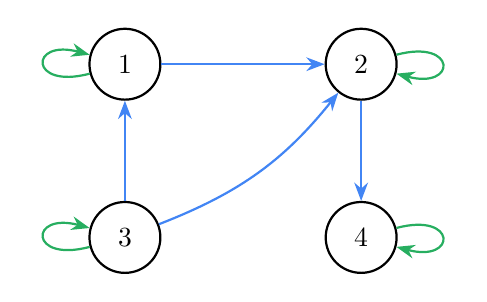
\begin{tikzpicture}[
  every node/.style={circle, draw, thick, minimum size=9mm, inner sep=0pt},
  >=Stealth
]
  \node (1) at (0,2.2)   {$1$};
  \node (2) at (3,2.2)   {$2$};
  \node (3) at (0,0)     {$3$};
  \node (4) at (3,0)     {$4$};

  % Original edges (blue)
  \draw[->, thick, setA] (1) -- (2);
  \draw[->, thick, setA] (3) -- (1);
  \draw[->, thick, setA] (3) edge[bend right=15] (2);
  \draw[->, thick, setA] (2) -- (4);
  % Added loops (green)
  \draw[->, thick, newEdge] (1) edge[loop left, looseness=8, min distance=8mm] (1);
  \draw[->, thick, newEdge] (2) edge[loop right, looseness=8, min distance=8mm] (2);
  \draw[->, thick, newEdge] (3) edge[loop left, looseness=8, min distance=8mm] (3);
  \draw[->, thick, newEdge] (4) edge[loop right, looseness=8, min distance=8mm] (4);
\end{tikzpicture}
\end{minipage}%
\begin{minipage}{0.45\textwidth}\centering
$M_{r(\alpha)} = \begin{pmatrix}
  \mathbf{1} & 1 & 0 & 0 \\
  0 & \mathbf{1} & 0 & 1 \\
  1 & 1 & \mathbf{1} & 0 \\
  0 & 0 & 0 & \mathbf{1}
\end{pmatrix}$

{\small\color{newEdge} Bold = added 1's on diagonal.}
\end{minipage}
\end{center}

%────────────────────────────────────────
\subsection*{Symmetric closure $s(\alpha)$}

Add the reverse of every pair:
\[
  \alpha^{-1} = \{(2,1),\,(1,3),\,(2,3),\,(4,2)\}.
\]
\[
  \boxed{s(\alpha) = \alpha \cup \alpha^{-1}
  = \{(1,2),\,(1,3),\,(2,1),\,(2,3),\,(2,4),\,(3,1),\,(3,2),\,(4,2)\}.}
\]

\begin{center}
\begin{minipage}{0.45\textwidth}\centering
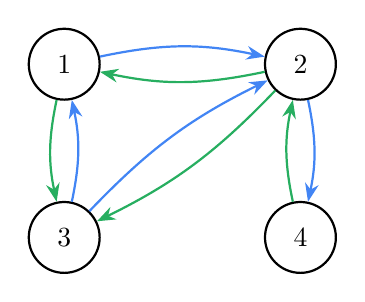
\begin{tikzpicture}[
  every node/.style={circle, draw, thick, minimum size=9mm, inner sep=0pt},
  >=Stealth
]
  \node (1) at (0,2.2)   {$1$};
  \node (2) at (3,2.2)   {$2$};
  \node (3) at (0,0)     {$3$};
  \node (4) at (3,0)     {$4$};

  % Original edges (blue) -- bend to make room for reverse
  \draw[->, thick, setA] (1) edge[bend left=12] (2);
  \draw[->, thick, setA] (3) edge[bend right=12] (1);
  \draw[->, thick, setA] (3) edge[bend left=10] (2);
  \draw[->, thick, setA] (2) edge[bend left=12] (4);
  % Added reverse edges (green)
  \draw[->, thick, newEdge] (2) edge[bend left=12] (1);
  \draw[->, thick, newEdge] (1) edge[bend right=12] (3);
  \draw[->, thick, newEdge] (2) edge[bend left=10] (3);
  \draw[->, thick, newEdge] (4) edge[bend left=12] (2);
\end{tikzpicture}
\end{minipage}%
\begin{minipage}{0.45\textwidth}\centering
$M_{s(\alpha)} = \begin{pmatrix}
  0 & 1 & \mathbf{1} & 0 \\
  \mathbf{1} & 0 & \mathbf{1} & 1 \\
  1 & 1 & 0 & 0 \\
  0 & \mathbf{1} & 0 & 0
\end{pmatrix}$

{\small\color{newEdge} Bold = added 1's ($M$ is now symmetric).}
\end{minipage}
\end{center}

%────────────────────────────────────────
\subsection*{Transitive closure $t(\alpha)$}

\textbf{Interpretation.}\; The transitive closure $t(\alpha)$ adds all pairs $(a,c)$ such that there is a directed path from $a$ to $c$ in the relation graph. Equivalently, $(a,c) \in t(\alpha)$ iff $a$ can reach $c$ in one or more steps.

\medskip

\begin{tcolorbox}[colback=yellow!5, colframe=stmtFrame!80, arc=2mm,
  fonttitle=\bfseries, title={\small Visual Build-Up: Adding ``Shortcut'' Edges},
  breakable, left=5pt, right=5pt, top=4pt, bottom=4pt]
The transitive closure is built layer by layer.  At each step we look for paths of increasing length and add a direct ``shortcut'' edge for each one.

\begin{center}
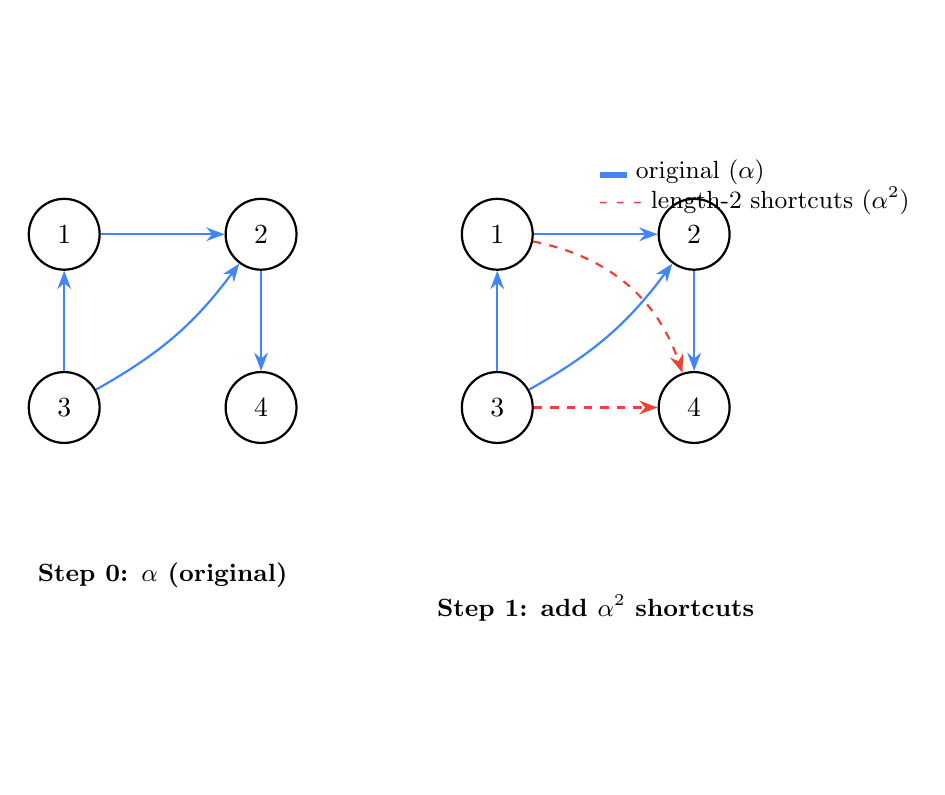
\begin{tikzpicture}[
  every node/.style={circle, draw, thick, minimum size=9mm, inner sep=0pt},
  >=Stealth
]
  % --- Layer 0: Original relation ---
  \begin{scope}[local bounding box=L0]
    \node (a1) at (0,2.2)   {$1$};
    \node (a2) at (2.5,2.2) {$2$};
    \node (a3) at (0,0)     {$3$};
    \node (a4) at (2.5,0)   {$4$};
    \draw[->, thick, setA] (a1) -- (a2);
    \draw[->, thick, setA] (a3) -- (a1);
    \draw[->, thick, setA] (a3) edge[bend right=12] (a2);
    \draw[->, thick, setA] (a2) -- (a4);
  \end{scope}
  \node[draw=none, below=2pt of L0, font=\small\bfseries] {Step 0: $\alpha$ (original)};

  % --- Layer 1: Add length-2 shortcuts ---
  \begin{scope}[xshift=5.5cm, local bounding box=L1]
    \node (b1) at (0,2.2)   {$1$};
    \node (b2) at (2.5,2.2) {$2$};
    \node (b3) at (0,0)     {$3$};
    \node (b4) at (2.5,0)   {$4$};
    % Original edges
    \draw[->, thick, setA] (b1) -- (b2);
    \draw[->, thick, setA] (b3) -- (b1);
    \draw[->, thick, setA] (b3) edge[bend right=12] (b2);
    \draw[->, thick, setA] (b2) -- (b4);
    % New shortcut edges (length-2 paths) -- dashed red
    \draw[->, thick, setB, dashed] (b1) edge[bend left=30] (b4);
    \draw[->, thick, setB, dashed] (b3) -- (b4);
  \end{scope}
  \node[draw=none, below=2pt of L1, font=\small\bfseries] {Step 1: add $\alpha^2$ shortcuts};

  % Legend
  \node[draw=none, font=\small, text width=4cm, align=left]
    at (8.8, 2.8) {%
      \textcolor{setA}{\rule{10pt}{2pt}} original ($\alpha$)\\
      \textcolor{setB}{- - -} length-2 shortcuts ($\alpha^2$)};
\end{tikzpicture}
\end{center}

\smallskip
In this example, vertex~$4$ is a sink (no outgoing edges), so there are \emph{no} paths of length~3 that produce new pairs.  The process terminates:  $t(\alpha) = \alpha \cup \alpha^2$.

In general, for $|A|=n$ the process always terminates after at most $n-1$ steps, since any path in an $n$-vertex graph that does not repeat vertices has length $\le n-1$.
\end{tcolorbox}

\medskip

We compute successive powers of $\alpha$:

\textbf{Step 1: $\alpha^2 = \alpha \circ \alpha$.}\; For each chain $x \xrightarrow{\alpha} y \xrightarrow{\alpha} z$:
\begin{itemize}[nosep]
  \item $(1,2)$ and $(2,4)$: gives $\boldsymbol{(1,4)}$.  \textbf{New!}
  \item $(3,1)$ and $(1,2)$: gives $(3,2)$.  Already in $\alpha$.
  \item $(3,2)$ and $(2,4)$: gives $\boldsymbol{(3,4)}$.  \textbf{New!}
\end{itemize}
New pairs: $\boxed{(1,4) \text{ and } (3,4)}$.

\textbf{Step 2: $\alpha^3 = \alpha^2 \circ \alpha$.}\; The new second coordinates are all~$4$, but $4$ has no outgoing edges in $\alpha$, so no further pairs arise.

\begin{answerbox}
$t(\alpha) = \alpha \cup \alpha^2 = \{(1,2),\;(1,4),\;(2,4),\;(3,1),\;(3,2),\;(3,4)\}.$
\end{answerbox}

\textbf{Interpretation:} $(x, z) \in t(\alpha)$ iff there is a directed path from $x$ to $z$ in the original digraph.

\begin{center}
\begin{minipage}{0.45\textwidth}\centering
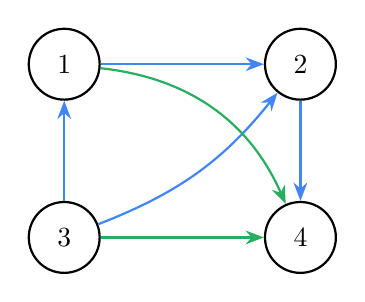
\begin{tikzpicture}[
  every node/.style={circle, draw, thick, minimum size=9mm, inner sep=0pt},
  >=Stealth
]
  \node (1) at (0,2.2)   {$1$};
  \node (2) at (3,2.2)   {$2$};
  \node (3) at (0,0)     {$3$};
  \node (4) at (3,0)     {$4$};

  % Original edges (blue)
  \draw[->, thick, setA] (1) -- (2);
  \draw[->, thick, setA] (3) -- (1);
  \draw[->, thick, setA] (3) edge[bend right=15] (2);
  \draw[->, thick, setA] (2) -- (4);
  % Added transitive edges (green)
  \draw[->, thick, newEdge] (1) edge[bend left=30] (4);
  \draw[->, thick, newEdge] (3) -- (4);
\end{tikzpicture}
\end{minipage}%
\begin{minipage}{0.45\textwidth}\centering
$M_{t(\alpha)} = \begin{pmatrix}
  0 & 1 & 0 & \mathbf{1} \\
  0 & 0 & 0 & 1 \\
  1 & 1 & 0 & \mathbf{1} \\
  0 & 0 & 0 & 0
\end{pmatrix}$

{\small\color{newEdge} Bold = added 1's.}
\end{minipage}
\end{center}

\medskip

\textbf{Reachability summary:}
\begin{itemize}[nosep]
  \item From $1$: can reach $2$ and $4$ \;(path: $1 \to 2 \to 4$).
  \item From $2$: can reach $4$.
  \item From $3$: can reach $1$, $2$, and $4$ \;(path: $3 \to 1 \to 2 \to 4$).
  \item From $4$: no outgoing edges --- $4$ is a \emph{sink}.
\end{itemize}

\end{document}
